%%
%% licence       kaneton licence
%%
%% project       kaneton
%%
%% file          /home/mycure/kaneton/view/papers/assignments/k1.tex
%%
%% created       matthieu bucchianeri   [tue feb  7 11:49:38 2006]
%% updated       julien quintard   [mon apr  3 01:45:53 2006]
%%

%
% k1
%

\section{k1}

%
% informations
%

\subsection{Informations}

\begin{tabular}{p{7cm}l}
Deadline: & XXX, 23h42 \\
Duration: & Two weeks \\
File name: & k1.tar.gz \\
In charge of: & Julien Quintard - \small{quinta\_j@epita.fr} \\
Newsgroups: & epita.cours.kaneton \\
Languages: & Assembly and C \\
Architectures: & Intel Architecture 32-bit \\
Students per group: & Three \\
\end{tabular}

%
% overview
%

\subsection{Overview}

The \textbf{k1} project consists in the development of the bootloader.

XXX

---
    For the bootloader, the only required fields of the \textit{o\_segment}
    structures are \textit{segid}, \textit{address}, \textit{size} and
    \textit{perms}.

    Other fields will be filled in at kernel initialization time.

    Note that the \textit{segid} field must be equal to the
    \textit{address} one.
---

---
    The bootloader must fill in the \textit{segid}, \textit{address},
    \textit{offset} and \textit{size} fields of each \textit{o\_region}
    structure.

    Since many segments will be needless, this array will only specify the
    fundamental segments to map.
---

%
% assignments
%

\subsection{Assignments}

In this project, the students have to develop the entire source code.
This means that no interface will be provided.

The only requirement is your bootloader to be compliant with the
initialization structure passed to the kaneton microkernel.

If this structure is not correctly built, then the kernel would not
be able to run.

Below are listed the bootloader's steps:

\begin{enumerate}
  \item
    The bootloader generally installs a more evolved memory addressing model,
    depending on the architecture.
  \item
    The bootloader relocates the stuffs needed by the future kernel
    execution and build the initialization structure.

    The stuff includes:

    \begin{itemize}
      \item
	The kernel code.
      \item
	The modules.
      \item
	The pre-reserved segments.
      \item
	The pre-reserved regions.
      \item
	The kernel stack.
      \item
	The alloc survival area.
    \end{itemize}
  \item
    Then, the booloader prepares the kernel stack and calls it providing
    to the kernel a complete initialization structure.
\end{enumerate}

The relocation is not really necessary but we wanted the students
to understand low-level programming and more especially programming
in a very strict environment with no fine-grain allocator provided.

The main goal of this project is to lead the students to understand the
project source organization. Indeed, a complete development environment
is provided; therefore, the students should learn to use system defines,
internal facilities etc.. to develop more quickly.

Displaying the initialization structure's information is the
minimum requirement. Having an enhanced display of pre-reserved
segments, regions and modules will be very appreciated, but is not required.

The code provided must be located in the directory
\textit{core/bootloader/arch/[architecture]/}.

\subsubsection{Tips}

Try to think about a very simple memory allocator delivering single
pages or contiguous areas. This allocator should help students to
allocate dynamic memory.

Assume that the kernel is the first given module.

\subsubsection{Additional Work}

Moreover, students should write a tiny console driver. Try to make this
driver code generic so you can reuse it in the next steps.

Finally, for this project, the students have to initialize the segment
and region manager, based on the segment and region array provided by
the bootloader's initialization structure. Note that this specific
initialization will change in the next projects.

\subsubsection{Bonus}

Be creative...

%
% ia32
%

\subsection{Intel Architecture 32-bit Implementation}

The bootloader is highly specific to the architecture because its main
roles are to:

\begin{itemize}
  \item
    Install new memory addressing models.
  \item
    Build the pre-reserved segment array.
  \item
    Build the pre-reserved region array.
\end{itemize}

The other tasks are independent of the architecture.

We will so detail the three previous points.

\subsubsection{Memory Addressing Models}

Since the kaneton microkernel can be implemented for three sub-architectures,
different Intel memory addressing models can be used.

We will assume in this document that the students implementing the
Intel architecture are using the \textit{ia32-virtual} architecture, meaning
that they are implementing the kaneton microkernel with true virtual memory.

Students willing implement kaneton with other specific Intel architecture
facilities should be able to adapt the assignments to their case.

So, in the case of the \textit{ia32-virtual} architecture, the bootloader
has to install two memory addressing models:

\begin{enumerate}
  \item
    First, the protected mode even if the bootstrap maybe installed it
    before.

    Indeed, the bootloader needs to rebuild the protected mode to be sure
    it is installed and to be able to maintain it.
  \item
    Then, the paging mode to enable virtual memory.
\end{enumerate}

We advise you to install the protected mode, then to relocate the stuff
and build the initialization structure and finally to install the
virtual memory before calling the kernel.

In this way, you will handle the hardest architecture problem, the virtual
memory, at the end, before performing the very last step, call the kernel.

\subsubsection{Segments}

The segment array passed to the kernel by the bootloader to the kernel via
the initialization structure is used to describe architecture dependent
physical memory areas as kaneton memory areas.

The kaneton memory areas are the logical memory areas to keep from being
erased like the kernel code, the kernel stack, the initialization structure,
the modules, the segment and region arrays, the survival area etc..

These areas, the core might be able to find out by itself but we prefer
specifying them in the segment array so everything is clear.

The architecture dependent memory areas are physical memory areas that
have a very special meaning on the running architecture. These area can
include the mapped video memory, the mapped BIOS ROM etc..

To keep the core segment manager from allocating memory on them, the
bootloader has to describe these areas via the segment array.

So the architecture dependent segments should include the ISA memory segment
and any other architecture specific reserved memory area for example for
the virtual memory page directories and page tables etc..

\subsubsection{Regions}

The region array must describe the virtual memory state on the specific
architecture for the kernel address space.

In other words, the region array must contains every virtual memory
areas in use once the region manager is initialized.

So, on the Intel architectures these include the mapped video memory,
the kernel code, the kernel stack, the initialization structure, the
survival area and any additional Intel specific objects like the Global
Descriptor Table etc..

Notice that it might be smart not to include the first memory page in
the region array. Mapping this page will cause null pointers to be valid!

\subsubsection{Example}

Below is a sample physical memory layout for the Intel architectures:

\begin{center}
  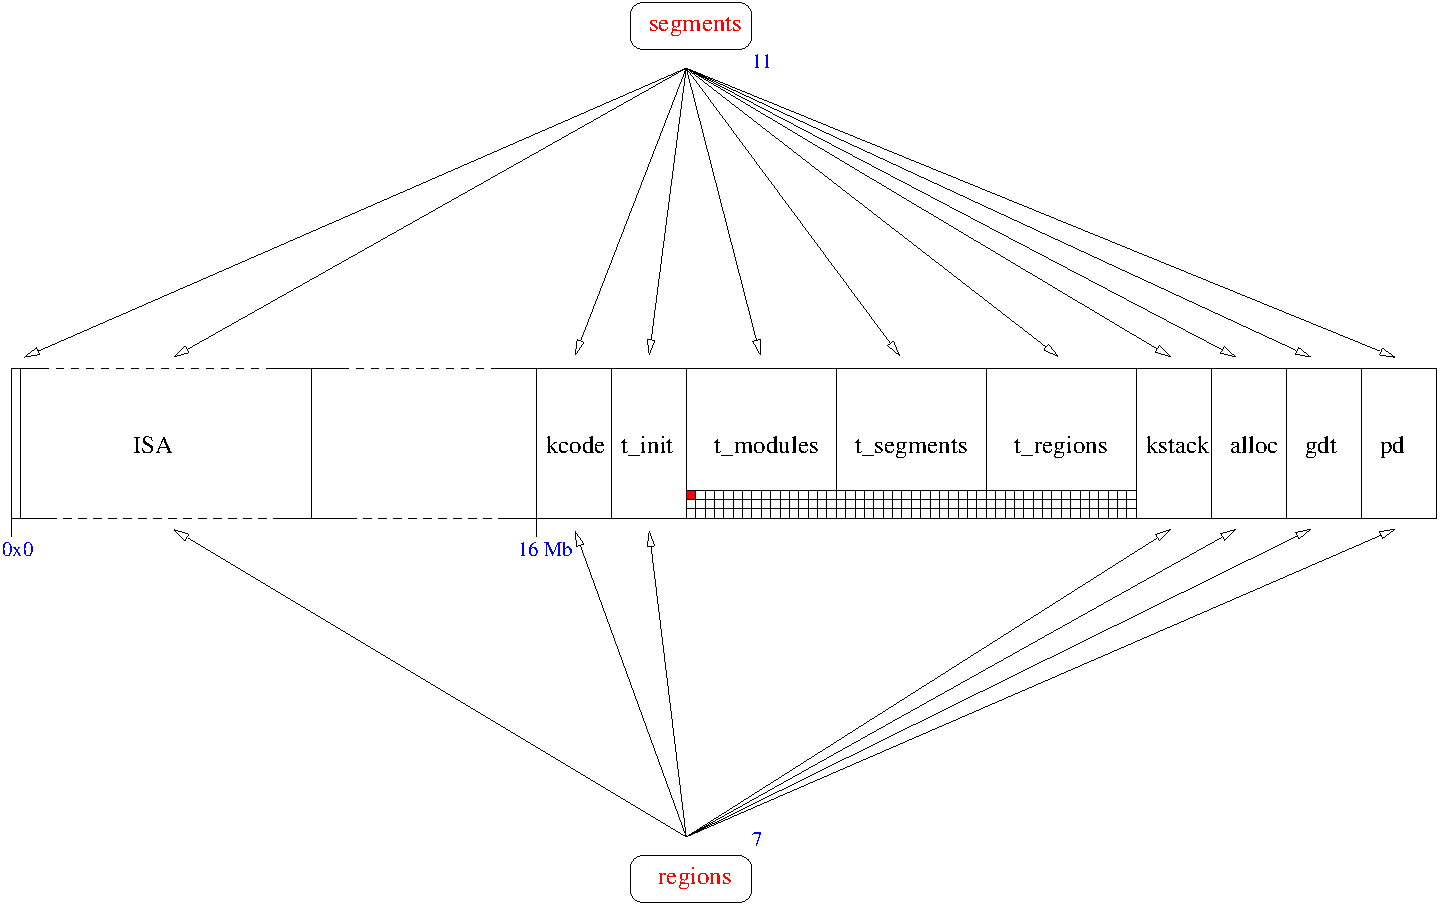
\includegraphics[scale=0.7]{figures/k1-memory-layout.pdf}
\end{center}
